\documentclass[11pt,aspectratio=169]{beamer}

%%==============================================================================
%% Header
%%==============================================================================

\usetheme{metropolis}
\usepackage{amsthm}
\newtheorem{ass}{Assumption}
\newtheorem{fac}{Fact}
\setsansfont{Source Sans Pro}
\setmonofont{Source Code Pro}

\hypersetup{colorlinks=true,
            linkcolor=mRustLightOrange,
            menucolor=mRustLightOrange,
            pagecolor=mRustLightOrange,
            urlcolor=mRustLightOrange}
\usepackage{csquotes}
\usepackage{comment}
\usepackage{xcolor}
\usepackage{minted}
\usepackage{pdfpages}
\usepackage{pdfcomment}
\usepackage{mathtools}
\usepackage{listings}

\definecolor{mRustDarkOrange}{HTML}{8d2f00}
\definecolor{mRustLightOrange}{HTML}{ff9600}
\definecolor{errMsg}{HTML}{CC1100}
\definecolor{warnMsg}{HTML}{EE9900}
\definecolor{refMsg}{HTML}{0011CC}
\definecolor{linkColor}{HTML}{002200}
\definecolor{urlColor}{HTML}{002200}
\hypersetup{colorlinks=true,linkcolor=linkColor,urlcolor=urlColor}

\let\orignote\note
\renewcommand<>{\note}[1]{\only#2{\tikz[remember,picture,overlay]{\node{\pdfmargincomment[opacity=0]{#1}}}}\orignote#2{#1}}

\AtBeginEnvironment{minted}{%
  \renewcommand{\fcolorbox}[4][]{#4}}

\newfontfamily\codefont{Source Code Pro}
\newcommand\code[1]{\,{\color[HTML]{884400}#1}\,}
\newcommand\source[1]{$\rightarrow$ via #1}

\title{Constant time algorithms in PQC}
\subtitle{\small{\url{https://lukas-prokop.at/talks/2022-01-26_rustgraz-const-time}}}
\date{\today}
\author{Lukas Prokop}
\institute{RustGraz community 
\includegraphics[height=.5cm]{../images/rustacean-orig-noshadow.png}}

\begin{document}
\maketitle

\label{ub}
\section{Introduction}

\begin{frame}[fragile]{Cryptography status-quo}
  \begin{minted}[fontsize=\tiny]{text}
$ nmap --script ssl-enum-ciphers -p 443 rust-lang.org
443/tcp open  https
| ssl-enum-ciphers: 
|   TLSv1.1: 
|     ciphers: 
|       TLS_ECDHE_RSA_WITH_AES_128_CBC_SHA (ecdh_x25519) - A
|       TLS_ECDHE_RSA_WITH_AES_256_CBC_SHA (ecdh_x25519) - A
|       TLS_RSA_WITH_AES_256_CBC_SHA (rsa 2048) - A
|       TLS_RSA_WITH_AES_128_CBC_SHA (rsa 2048) - A
|       TLS_ECDHE_RSA_WITH_AES_128_GCM_SHA256 (ecdh_x25519) - A
|       TLS_ECDHE_RSA_WITH_AES_128_CBC_SHA256 (ecdh_x25519) - A
|       TLS_ECDHE_RSA_WITH_AES_256_GCM_SHA384 (ecdh_x25519) - A
|       TLS_ECDHE_RSA_WITH_CHACHA20_POLY1305_SHA256 (ecdh_x25519) - A
|       TLS_ECDHE_RSA_WITH_AES_256_CBC_SHA384 (ecdh_x25519) - A
|       TLS_RSA_WITH_AES_128_GCM_SHA256 (rsa 2048) - A
|       TLS_RSA_WITH_AES_256_GCM_SHA384 (rsa 2048) - A
|       TLS_RSA_WITH_AES_128_CBC_SHA256 (rsa 2048) - A
|     compressors: 
|       NULL
|     cipher preference: server
|   TLSv1.2: 
|     ciphers: 
|       TLS_ECDHE_RSA_WITH_AES_128_GCM_SHA256 (ecdh_x25519) - A
|       TLS_ECDHE_RSA_WITH_AES_128_CBC_SHA256 (ecdh_x25519) - A
|       TLS_ECDHE_RSA_WITH_AES_128_CBC_SHA (ecdh_x25519) - A
|       TLS_ECDHE_RSA_WITH_AES_256_GCM_SHA384 (ecdh_x25519) - A
|       TLS_ECDHE_RSA_WITH_CHACHA20_POLY1305_SHA256 (ecdh_x25519) - A
|       TLS_ECDHE_RSA_WITH_AES_256_CBC_SHA384 (ecdh_x25519) - A
|       TLS_ECDHE_RSA_WITH_AES_256_CBC_SHA (ecdh_x25519) - A
|       TLS_RSA_WITH_AES_128_GCM_SHA256 (rsa 2048) - A
|       TLS_RSA_WITH_AES_256_GCM_SHA384 (rsa 2048) - A
|       TLS_RSA_WITH_AES_128_CBC_SHA256 (rsa 2048) - A
|       TLS_RSA_WITH_AES_256_CBC_SHA (rsa 2048) - A
|       TLS_RSA_WITH_AES_128_CBC_SHA (rsa 2048) - A
|     compressors: 
|       NULL
|     cipher preference: server
|_  least strength: A
  \end{minted}
\end{frame}


\begin{frame}[fragile]{Post-quantum cryptography (PQC)}
  \begin{fac}
    Our current cryptographic infrastructure is built on top of RSA and elliptic cryptography.
    Their security is based on the integer factorization (RSA) and discrete logarithm problem (ECC).
  \end{fac}
  \begin{ass}
    A sufficiently large quantum computer can solve integer factorization and the discrete logarithm problem in polynomial time (c.f. Shor's algorithm, Grover's algorithm).
  \end{ass}
  \begin{ass}
    No sufficiently large quantum computer exists, but we should protect current communication against future decryption.
  \end{ass}
\end{frame}

\begin{frame}[fragile]{Post-quantum cryptography (PQC)}
  \emph{Research questions:}
  \begin{enumerate}
    \item Which problems provide security under the QROM model?
    \item Which cryptographic primitives do we need?
    \item What are algorithmic candidates for cryptographic primitives?
    \item Which algorithms can be implemented [securely and efficiently] in software and hardware?
  \end{enumerate}
\end{frame}

\begin{frame}[fragile]{Post-quantum cryptography (PQC)}
  \emph{Basic answers:}
  \begin{description}
    \item[problems] Speculation. Ask theoretical computer scientists about the presumed difficulty to solve computational problems.
    \item[primitives] Symmetric cryptographic primitives can be used with doubled key sizes. Asymmetric cryptographic primitives like public key encryption schemes and digital signatures need to be replaced.
    \item[candidates] Ask cryptographic community for proposals. Ask everyone to break security.
    \item[implementation] Ask for feedback within a time frame.
  \end{description}
\end{frame}

\begin{frame}[fragile]{Post-quantum cryptography (PQC)}
  Initiate cryptograpic competition\footnote{\enquote{\href{https://eprint.iacr.org/2020/1608.pdf}{Cryptographic competitions}} by Daniel J. Bernstein (2020)} similar to SHA-3, CAESAR, and NISTLWC.

  Competition by National Institute for Standards and Technology, USA (NIST)
  \begin{description}
    \item[2016-02] Announcement for \enquote{Post-Quantum Cryptography Standardization Effort}
    \item[2017-11] Deadline for submissions
    \item[2017-12] Round 1 algorithms announced (69)
    \item[2019-01] Round 2 algorithms announced (26)
    \item[2020-07] Round 3 algorithms announced (7)
    \item[2022-01] Schemes to standardize to be announced
    \item[2024] Expected end of standardization
  \end{description}
\end{frame}

\begin{frame}[fragile]{Post-quantum cryptography (PQC)}
  \emph{What are candidates for post-quantum cryptography NOT?}
  \begin{itemize}
    \item New algorithms for symmetric algorithms
    \item Quantum cryptography: Industry won't be able to deploy quantum co-processors in the next few years.
  \end{itemize}

  \emph{Common approach:}
  \begin{enumerate}
    \item Pick an NP-hard problem, where no advantage is known for quantum computers.
    \item Design cryptographic scheme on top of the problem
    \item Reiterate over implementations to improve efficiency and security
  \end{enumerate}
\end{frame}

\begin{frame}[fragile]{Cryptographic primitives}
  Key Encapsulation Mechanism:
  \begin{enumerate}
    \item KeyGen() → (pk, sk)
    \item Encapsulate(pk) → (ct, ss)
    \item Decapsulate(pk, sk, ct) → (ss)
  \end{enumerate}

  Digital signatures:
  \begin{enumerate}
    \item KeyGen() → (pk, sk)
    \item Sign(sk, msg) → (sig)
    \item Verify(sig, msg, pk) → (msg)
  \end{enumerate}
\end{frame}  

\begin{frame}[fragile]{PQC Round 3 finalists}
  \begin{center}
    {\scriptsize\url{https://csrc.nist.gov/projects/post-quantum-cryptography/round-3-submissions}} \\
    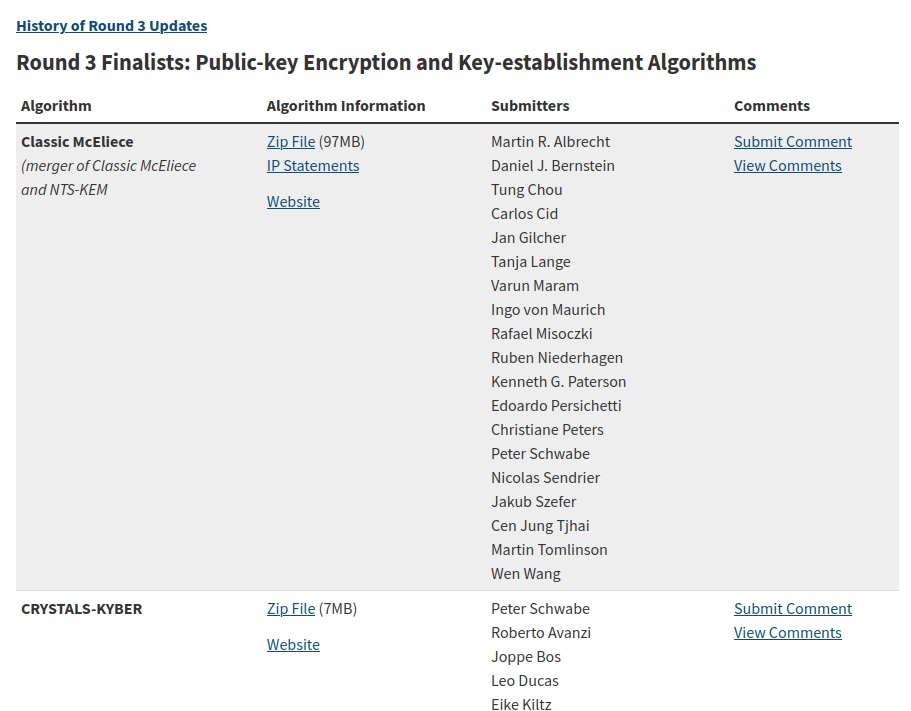
\includegraphics[width=220px]{images/pqc-round3-screenshot.png}
  \end{center}
\end{frame}


\begin{frame}[fragile]{PQC Round 3 finalists}
  \href{https://csrc.nist.gov/projects/post-quantum-cryptography/round-3-submissions}{Round 3 finalists}:
  \begin{enumerate}
    \item Classic McEliece (KEM, code)
    \item CRYSTALS-KYBER (KEM, lattice, MLWE)
    \item NTRU (KEM, lattice, NTRU)
    \item SABER (KEM, lattice, MLWR)
    \item CRYSTALS-DILITHIUM (sig, lattice, Fiat-Shamir)
    \item FALCON (sig, lattice, NTRU)
    \item Rainbow (sig, multi-variate, Oil-Vinegar)
  \end{enumerate}
  (Alternate candidates neglected)

  \textbf{General categories:} lattice-based, code-based, multivariate, hash-based, braid group, supersingular elliptic curve cryptography
\end{frame}

\section{Usecase}

\begin{frame}[fragile]{Security}
  \begin{description}
    \item[Theoretical security] choice of parameters
    \item[Software security] timing, caches, memory management, \\ misuse prevention by API design
    \item[Hardware security] EM emission, power analysis, fault attacks
  \end{description}
\end{frame}

\begin{frame}[fragile]{Security}
  \begin{description}
    \item[Theoretical security] choice of parameters
    \item[Software security] \underline{timing}, caches, memory management, \\ misuse prevention by API design
    \item[Hardware security] EM emission, power analysis, fault attacks
  \end{description}
\end{frame}
  
\begin{frame}[fragile]{Constant time}
  \begin{itemize}
    \item On our hardware, assembly instructions are run
    \item Independent of the values, the algorithm should take the same amount of time (i.e. constant time)
    \item Classic counterexample: \href{https://en.wikipedia.org/wiki/Exponentiation_by_squaring}{Exponentiation by squaring}
    \item Sorry, most code snippets are in C
  \end{itemize}
\end{frame}

\begin{frame}[fragile]{Assembly in rust}
  \href{https://www.lukas-prokop.at/articles/2021-11-10-rdtsc-with-rust-asm}{Blog article \enquote{Intel's RDTSC instruction with rust's RFC-2873 asm! macro} (2021)}
  \begin{minted}[fontsize=\small]{rust}
#![feature(asm)]

#[cfg(any(target_arch = "x86", target_arch = "x86_64"))]
fn has_rdtsc_support() -> bool {
  // Step 1: ask for generic information and print it to stdout
  {
    let ebx: u32;
    let ecx: u32;
    let edx: u32;
  \end{minted}
\end{frame}

\begin{frame}[fragile]{Assembly in rust}
  \href{https://www.lukas-prokop.at/articles/2021-11-10-rdtsc-with-rust-asm}{Blog article \enquote{Intel's RDTSC instruction with rust's RFC-2873 asm! macro} (2021)}
  \begin{minted}[fontsize=\scriptsize]{rust}
unsafe {
  asm!(
    "cpuid",
    "mov {bx:e}, ebx",
    // “output operands” following
    bx = lateout(reg) ebx,
    lateout("ecx") ecx,
    lateout("edx") edx,
    // “input operands” following
    in("eax") 0,
    // “clobbers” list
    lateout("eax") _,
    // “options” ∈ {"pure", "nomem", "nostack"}
    options(nomem, nostack)
  );
}
  \end{minted}
\end{frame}

\begin{frame}[fragile]{Software security}
  \begin{itemize}
    \item branch instructions independent of the secret
    \item memory access pattern independent of the secret
    \item runtime independent of the secret (constant time algorithms)
  \end{itemize}
  \textit{Various countermeasures in physical security:} \\
  Masking, shuffling, randomized instruction order, \dots{}

  \textit{Various countermeasures in software security:} \\
  Branch independence, indexing independent of secret, prevention of data races, \dots{}
\end{frame}

\section{Constant time algorithms}

\begin{frame}[fragile]{argument is non-zero}
  \textbf{Problem:} Let $a$ be integer $\in \{0, \dots, 15\}$. Return 0 if $a=0$ else $1$.
  \begin{minted}{C}
static inline uint8_t gf16_is_nonzero(uint8_t a) {
  unsigned a4 = a & 0xf;
  unsigned r = ((unsigned) 0) - a4;
  r >>= 4;
  return r & 1;
}
\end{minted}
  via Rainbow round 3 reference implementation, \verb=gf16.c=
\end{frame}

\begin{frame}[fragile]{Reminder: two's complement}
  \textit{How does one represent non-negative integer $i$ bitwise?} \\
  Value $0$ is a sequence of zeros. Value $1$ has the least-significant bit (LSB) zero but others set to one (i.e. \dots{}0001). Value 2 is represented as \dots{}0010. And so on \dots{}

  \textit{How does one represent $-i$ for non-negative integer $i$ bitwise?} \\
  The most common encoding used on all platforms is the \href{https://en.wikipedia.org/wiki/Two%27s_complement}{two's complement}:
  If we map value $i$ to the negative space, we need to invert all bits and add 1. Example: \dots{}0001 inverted, gives \dots{}1110 and adding 1 gives \dots{}1111. Thus, $-1$ is a sequence of ones.
\end{frame}

\begin{frame}[fragile]{argument is non-zero}
  \textbf{Description:}
  \begin{itemize}
    \item recognize that $a4$ (unlike $a$) has more than 8 bits.
    \item if $a$ is zero
      \begin{itemize}
        \item then $0-0$ yields zero for $r$
        \item the fourth bit of $r$ is zero
        \item returns 0
      \end{itemize}
    \item else
      \begin{itemize}
        \item $a4$ has 4 bits set
        \item the two's complement by $0-a4$ sets the fifth, sixth, \dots{} bits to one
        \item the fourth bit of $r$ is one
        \item returns 1
      \end{itemize}
  \end{itemize}
\end{frame}

\begin{frame}[fragile]{conditional move}
  \textbf{Problem:} If $b=1$, copy \textsf{len} elements from \textsf{x} to \textsf{r}. If $b=0$, don't do anything.
  \begin{minted}{C}
/* b = 1 means mov, b = 0 means don't mov*/
void cmov(unsigned char *r, const unsigned char *x,
          size_t len, unsigned char b)
{
  size_t i;

  b = (~b + 1);
  for(i=0;i<len;i++)
    r[i] ^= b & (x[i] ^ r[i]);
}
\end{minted}
  via Classic McEliece round 3 reference implementation, \verb=int32_sort.c=
\end{frame}

\begin{frame}[fragile]{Reminder: XOR}
  \begin{itemize}
    \item XOR is denoted by the \verb=^= operator
    \item XOR is a bitwise binary operator and returns 1 iff both bits are different
    \item \verb=a ^ b= for some integers $a$ and $b$ is zero iff $a$ equals $b$
    \item \verb=a ^ a= for some integer $a$ is always zero
  \end{itemize}
\end{frame}

\begin{frame}[fragile]{conditional move}
  \textbf{Description:}
  \begin{itemize}
    \item recognize that $b$ is (two's complement) negated first.
    \item thus, if $b$ is zero, it retains zero. Otherwise $b$ becomes a sequence of ones bits ($-1$).
    \item if $b$ is zero
      \begin{itemize}
        \item we compute \mintinline{rust}{r[i] = r[i] ^ 0}
      \end{itemize}
    \item if $b$ is a sequence of ones bits
      \begin{itemize}
        \item we compute \mintinline{rust}{r[i] = r[i] ^ (x[i] ^ r[i])}
        \item this equals \mintinline{rust}{r[i] = (r[i] ^ r[i]) ^ x[i]}
        \item this equals \mintinline{rust}{r[i] = 0 ^ x[i] = x[i]}
      \end{itemize}
  \end{itemize}
\end{frame}

\begin{frame}[fragile]{modulo 3}
  \textbf{Problem:} Compute $a \bmod{3}$ of some integer $a \in \{0, 1, \dots, 2^{13}-1\}$.

  \href{https://www.lukas-prokop.at/articles/2021-06-15-modulo}{Blog article \enquote{Deriving algorithms for computing modulo constant n} (2021)} \\
  \href{https://www.lukas-prokop.at/articles/2021-06-16-mod3}{Blog article \enquote{mod3 of NTRU's reference implementation} (2021)}
  \begin{minted}[fontsize=\scriptsize]{C}
static uint16_t mod3(uint16_t a)
{
  uint16_t r;
  int16_t t, c;
  r = (a >> 8) + (a & 0xff); // r mod 255 == a mod 255
  r = (r >> 4) + (r & 0xf); // r' mod 15 == r mod 15
  r = (r >> 2) + (r & 0x3); // r' mod 3 == r mod 3
  r = (r >> 2) + (r & 0x3); // r' mod 3 == r mod 3

  t = r - 3;
  c = t >> 15;
  return (c&r) ^ (~c&t);
}
\end{minted}
  via NTRU round 3 reference implementation \verb=sample_iid.c=
\end{frame}

\begin{frame}[fragile]{modulo 3}
  \textbf{Rough description (blog articles contain details):}
  \begin{itemize}
    \item in general, ‘$(a \bmod{kp}) \bmod{p}$’ equals ‘$a \bmod{p}$’ where $a, k, p \in \mathbb Z$
    \item $15$ and $255$ are multiples of $3$
    \item the first three assignments $r$ use this principle to reduce mod $3$, but not completely
    \item after the first three assignments, $r \in \{0, 1, \dots, 5\}$ with $r \equiv a \bmod{3}$
    \item so, $t \in \{-3, -2, \dots, 2\}$
    \item $c$ is 0 if $t$ is negative and $1$ otherwise
    \item we return $r$ if $c$ is zero, otherwise $t$
  \end{itemize}
\end{frame}

\begin{frame}[fragile]{0,1,2 to 0,1,q-1}
  \textbf{Problem:} Given a polynomial $r$ with coefficients $\in \{0,1,2\}$. Map them to $\{0,1,\textsf{NTRU\_Q}-1\}$ assuming the three LSBs of $\textsf{NTRU\_Q}-1$ are ones.
  \begin{minted}[fontsize=\small]{C}
/* Map {0, 1, 2} -> {0,1,q-1} in place */
void poly_Z3_to_Zq(poly *r)
{
  int i;
  for(i=0; i<NTRU_N; i++)
    r->coeffs[i] = r->coeffs[i]
                 | ((-(r->coeffs[i]>>1)) & (NTRU_Q-1));
}
\end{minted}
  via NTRU round 3 reference implementation \verb=poly.c=
\end{frame}

\begin{frame}[fragile]{0,1,2 to 0,1,q-1}
  \textbf{Description:}
  \begin{itemize}
    \item \mintinline{rust}{r->coeffs[i]>>1} is 0 for values $\{0,1\}$ and $1$ for $\{2\}$
    \item \mintinline{rust}{-(r->coeffs[i]>>1)} is 0 for values $\{0,1\}$ and a sequence of ones for $\{2\}$
    \item if the value is $0$ or $1$, we apply AND to 0 and $\textsf{NTRU\_Q}-1$ which is 0
    \item if the value is $2$, we apply AND to $-1$ and $\textsf{NTRU\_Q}-1$ which is $\textsf{NTRU\_Q}-1$
  \end{itemize}
\end{frame}

\begin{frame}[fragile]{minmax}
  \textbf{Problem:} Given 31-bit integers $a$ and $b$. Assign $a = \operatorname{min}(a,b)$ and $b = \operatorname{max}(a,b)$
  \begin{minted}{C}
#define int32_MINMAX(a,b) \
do { \
  int32_t ab = b ^ a; \
  int32_t c = b - a; \
  c ^= ab & (c ^ b); \
  c >>= 31; \
  c &= ab; \
  a ^= c; \
  b ^= c; \
} while(0)
  \end{minted}
\end{frame}

\begin{frame}[fragile]{minmax}
  \textbf{Description:}
  \begin{itemize}
    \item $c$ is positive if $b \geq a$ and negative otherwise
    \item 32nd bit of $c$ indicates whether we need to swap
    \item A right-shift operator for signed integers replicates the most-significant bit. So, \mintinline{rust}{0b1000_0000i8 >> 7 == 0b1111_1111}
    \item so we apply AND between $c$ and \mintinline{rust}{b ^ a}
    \item If $a \geq b$, \mintinline{rust}{a = a ^ ab = a ^ b ^ a = b} \\
          else $a < b$, \mintinline{rust}{a = a ^ ab = a ^ 0 = a}
  \end{itemize}

  This code is the fundamental routine for conditional swaps to implement sorting algorithms.
  To implement sorting algorithms in constant time, you need algorithms similar to merge sort (c.f. TAOCP, Vol 3, sorting networks).
\end{frame}

\begin{frame}[fragile]{number of trailing zeros of the non-zero input in}
  \textbf{Description:} Count the number of zero bits next to the LSB (\enquote{trailing zeros})
  \begin{minted}{C}
static inline int ctz(uint64_t in) {
  int i, b, m = 0, r = 0;

  for (i = 0; i < 64; i++) {
    b = (in >> i) & 1;
    m |= b;
    r += (m^1) & (b^1);
  }

  return r;
}
  \end{minted}
  via Classic McEliece round 3 reference implementation, \verb=pk_gen.c=
\end{frame}

\begin{frame}[fragile]{number of trailing zeros of the non-zero input in}
  \textbf{Description:}
  \begin{itemize}
    \item $b$ contains the $i$-th bit of variable in
    \item $m$ is one iff $b$ is one or any bit before is one
    \item $r$ is a counter
    \item Assume the LSB is zero, then $b$ is zero, $m$ is zero. \mintinline{rust}{(0^1) & (0^1) = 1 & 1 = 1}.
    \item Assume the LSB is one, then $b$ is one, $m$ is one. \mintinline{rust}{(1^1) & (1^1) = 0 & 0 = 0}.
    \item If a consecutive bit is zero, but a previous bit was one, one element of the AND operation becomes zero and thus zero will be added to $r$.
  \end{itemize}
\end{frame}

\section{Audience quiz}


\begin{frame}[fragile]{Problem statement}
  \begin{minted}{C}
static inline unsigned char same_mask(uint16_t x, uint16_t y);
  \end{minted}
  \textbf{Problem:} If $x$ equals $y$, return non-zero. If $x$ does not equal $y$, return zero.

  \textbf{Goal:} write a constant time algorithm.
\end{frame}

\begin{frame}[fragile]{Solution}
  \begin{minted}{C}
static inline unsigned char same_mask(uint16_t x, uint16_t y)
{
  uint32_t mask;

  mask = x ^ y;
  mask -= 1;
  mask >>= 31;
  mask = -mask;

  return mask & 0xFF;
}
\end{minted}
  via Classic McEliece round 3 reference implementation, \verb=pk_gen.c=
\end{frame}


% TODO David wants to hold next talk

\begin{frame}[standout]
  \begin{center}
    \vspace{1.5cm}
    Thank you! Q/A?

    
\includegraphics[width=0.4\textwidth]{../images/rustacean-flat-happy.png}
  \end{center}
\end{frame}

\begin{frame}[fragile]{Advertisment}
  \textbf{Grazer Linuxtage:}
  \begin{itemize}
    \item https://www.linuxtage.at/en/
    \item Fri, 2022-04-22 and Sat, 2022-04-23
    \item On-site event at TU Graz Inffeld
    \item Please submit your \href{https://pretalx.linuxtage.at/glt22/cfp}{proposal}!
  \end{itemize}
\end{frame}

\end{document}
